\section{Kolineární geometrie} \label{kap_kolinearni}
V kolineární geometrii jsme provedli tři druhy měření hysterezních smyček. 
\begin{itemize}
\item Polarizační závislost pro $\phH=\ang{135}$ a $T<\SI{15}{\kelvin}$ pro ověření funkčnosti a porovnání s nekolineární geometrií.
\item Závislost na směru vnějšího pole $\phH \in (\ang{0},\ang{360})$ při $T<\SI{15}{\kelvin}$ a fixovaném $\gamma-\beta=\ang{90}$ (maximální Voigtův jev a nulové MLD).
\item Teplotní závislost pro $\phH=\ang{135}$ a fixované polarizaci $\beta=\ang{0}$ (maximální Voigtův jev a nulové MLD).
\end{itemize}


\subsection{Polarizační závislost při vnějším poli ve směru \ang{135}}
Měření proběhlo při teplotě $T<\SI{15}{\kelvin}$ a intenzita laseru dopadajícího na vzorek byla \SI{2}{\milli\watt}.

Na obr. \ref{kol_vysledky_voigt} (a) je typický průběh Voigtova jevu. Na obr. \ref{kol_vysledky_voigt} (b) jsou hysterezní smyčky pro několik vybraných polarizací. Polarizační závislost amplitudy přeskoku $A$ je vykreslena na obr. \ref{kol_vysledky_voigt} (c). V tabulce \ref{tab_kol_hyst135} jsou shrnuté získané výsledky.

\begin{figure}[htbp]\centering
\qq{	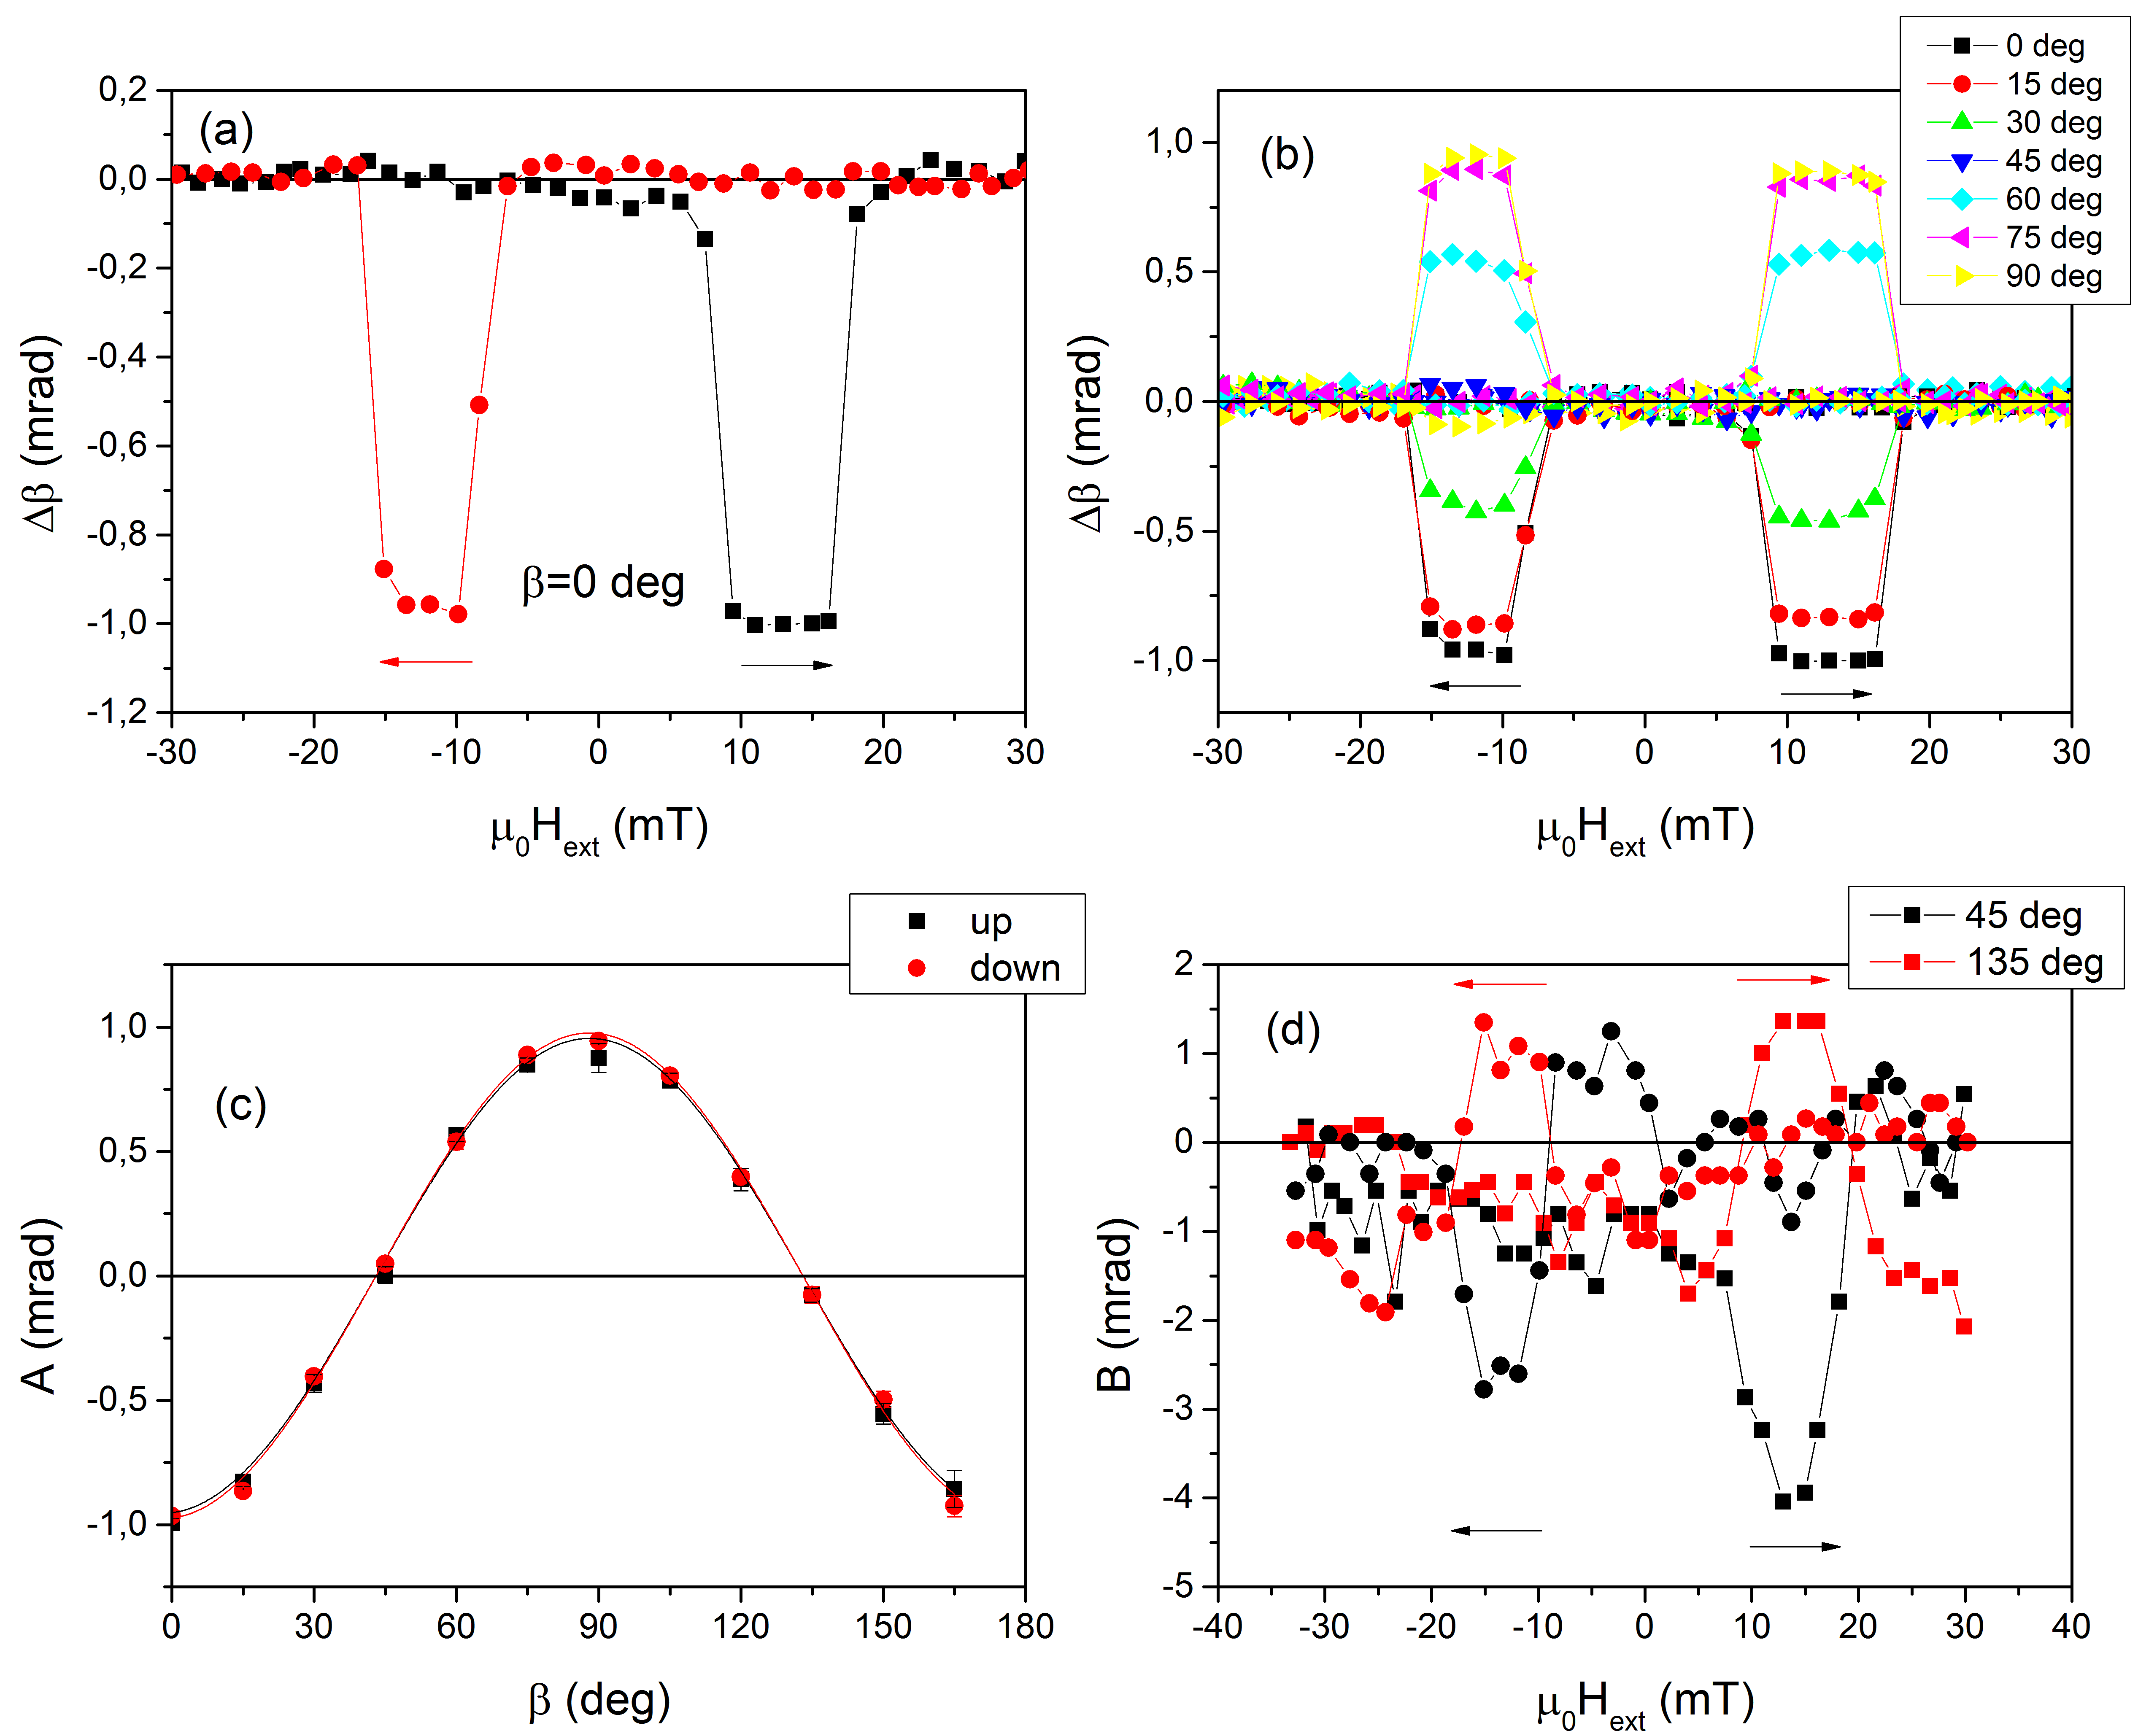
\includegraphics[width=\textwidth]{./png/kolhyst_135pol}}
	\caption{Měření Voigtova jevu v hysterezních smyčkách pro $\phH=\ang{135}$ v~kolineární geometrii. (a) Typická hysterezní smyčka ($\beta=\ang{0}$). (b) Polarizační závislost hysterezních smyček. (c) Polarizační závislost amplitudy $A$ (body), nafitovaná závislost vztahem \eqref{e:amplVoigt} (čára). (d) Součtový signál pro vybrané polarizace.}\label{kol_vysledky_voigt}
\end{figure}

\begin{table}[htbp]	
	\centering	
	\begin{tabular}{c||cc|cc}
		& & & \multicolumn{2}{c}{fit Voigtův jev} \\
		 & $\mu_0\hcj$ & $\mu_0\hcd$ & $\pmld \sin\xi$ & $\gamma$ \\
		 & (mT) & (mT) & (\si{\milli\radian}) & (deg)  \\ \hline
		up & \num{6,8(4)} & \num{17,6(6)} & \num{-0,48(4)} & \num{88,1(15)} \\
		down & \num{7,1(6)} & \num{16,5(7)} & \num{-0,49(3)} & \num{88,1(10)} \\
	\end{tabular}
	\caption{Měření hysterezních smyček v kolineární geometrii pro $\phH=\ang{135}$. Změnili jsme znaménko $\pmld \sin\xi$, protože dochází k přeskoku v opačném směru než předpokládá vztah \eqref{e:amplVoigt}}
	\label{tab_kol_hyst135}
\end{table}

V součtovém signálu je sice patrný MLD signál, ale je téměř na úrovni šumu a tak ho nezpracováváme, viz obr. \ref{kol_vysledky_voigt} (d). Vybrané polarizace jsou ty, u kterých by MLD mělo být nejsilnější.

Ve srovnání s měřením v nekolineární geometrii (viz obr. \ref{kol_nekol}) je patrné, že toto měření proběhlo při vyšší teplotě (viz níže). Koercitivní pole jsou nižší a $|\pmld|$ také. To mohlo být způsobeno, kromě odlišného zchlazení vzorku kryostatem, také vyšším výkonem použitého laseru.

\begin{figure}[htbp]\centering
\qq{	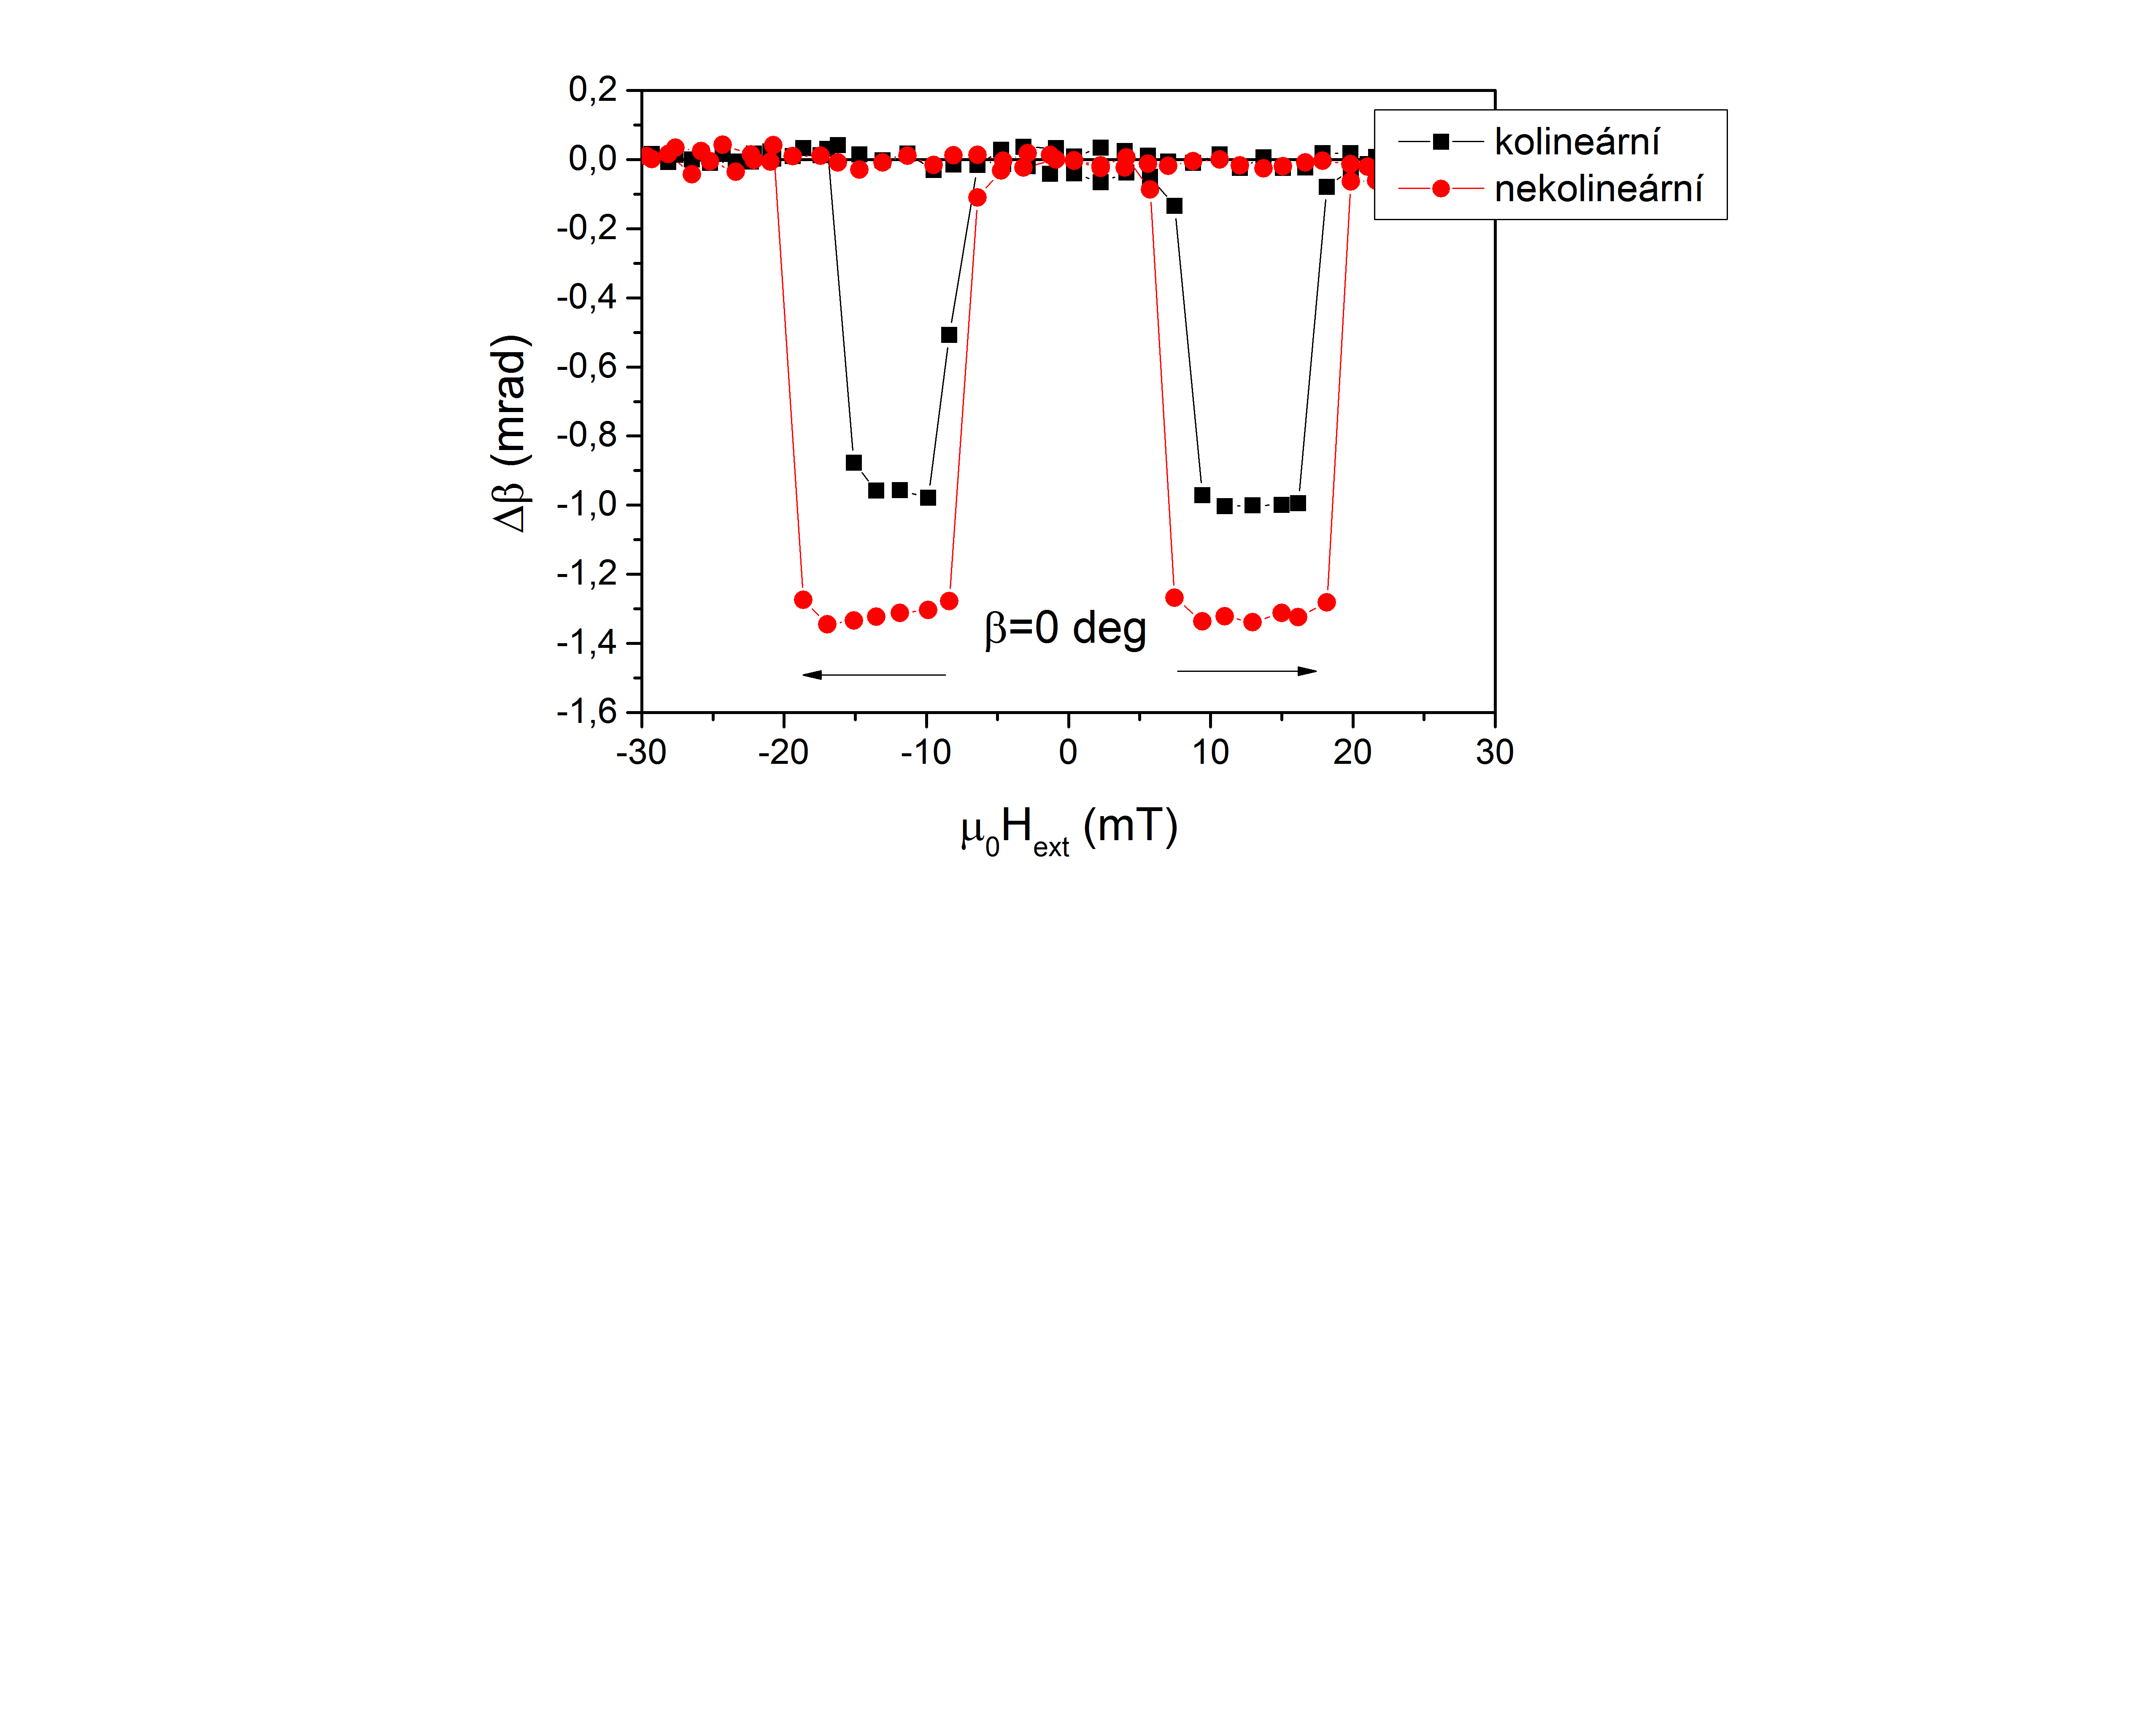
\includegraphics[trim={0 3.43in 0 0}, clip, width=\textwidth]{./png/kolhyst_nekol}}
	\caption{Porovnání Voigtova jevu v kolineární a nekolineární geometrii. Měření v kolineární geometrii pravděpodobně proběhla při vyšší teplotě.}\label{kol_nekol}
\end{figure}


\subsection{Závislost na směru vnějšího pole} \label{kap_smer}

Měřili jsme hysterezní smyčky ve všech směrech pole s krokem \ang{15}. Ovládání elektromagnetu má v současné době implementované a zkalibrované pouze čtyři směry: \ang{0}, \ang{45}, \ang{90}, \ang{135}. Zbývajících směrů jsme dosáhli otočením ramena kryostatu se vzorkem o $+\ang{15}$ a $-\ang{15}$. Zároveň se vzorkem jsme točili i rovinu polarizace, aby byla splněna podmínka $\gamma-\beta=\ang{90}$ a Voigtův jev byl maximální.
Směry $\phH>\ang{165}$ jsme měřili jako \emph{down} opačného směru.

Měření proběhlo při teplotě $T<\SI{15}{\kelvin}$ a intenzita laseru dopadajícího na vzorek byla \SI{1,2}{\milli\watt}.

U hysterezních smyček sledujeme veličiny $\hcj$, $\hcd$ a $A$ (viz obr. \ref{kol_okolo}).
Ve směrech \ang{45}, \ang{60}, \ang{225}, \ang{240} jsme nepozorovali žádný magnetooptický signál, protože magnetizace v průběhu hysterezní smyčky zjevně přeskakuje pouze mezi dvěma protilehlými snadnými osami. To je v souladu s očekávanou polohou prvnní snadné osy v tomto vzorku (viz tabulka \ref{tab_vzorek}), která při zvoleném nalepení (viz obr. \ref{souradna_soustava_vzorek}) odpovídá směru $59(5)^\circ$. Překvapivý je ale fakt, že při položení pole ve směru druhé snadné osy, který by se měla nacházet na poloze $121(5)^\circ$, smyčky pozorujeme.

\begin{figure}[htbp]\centering
\qq{	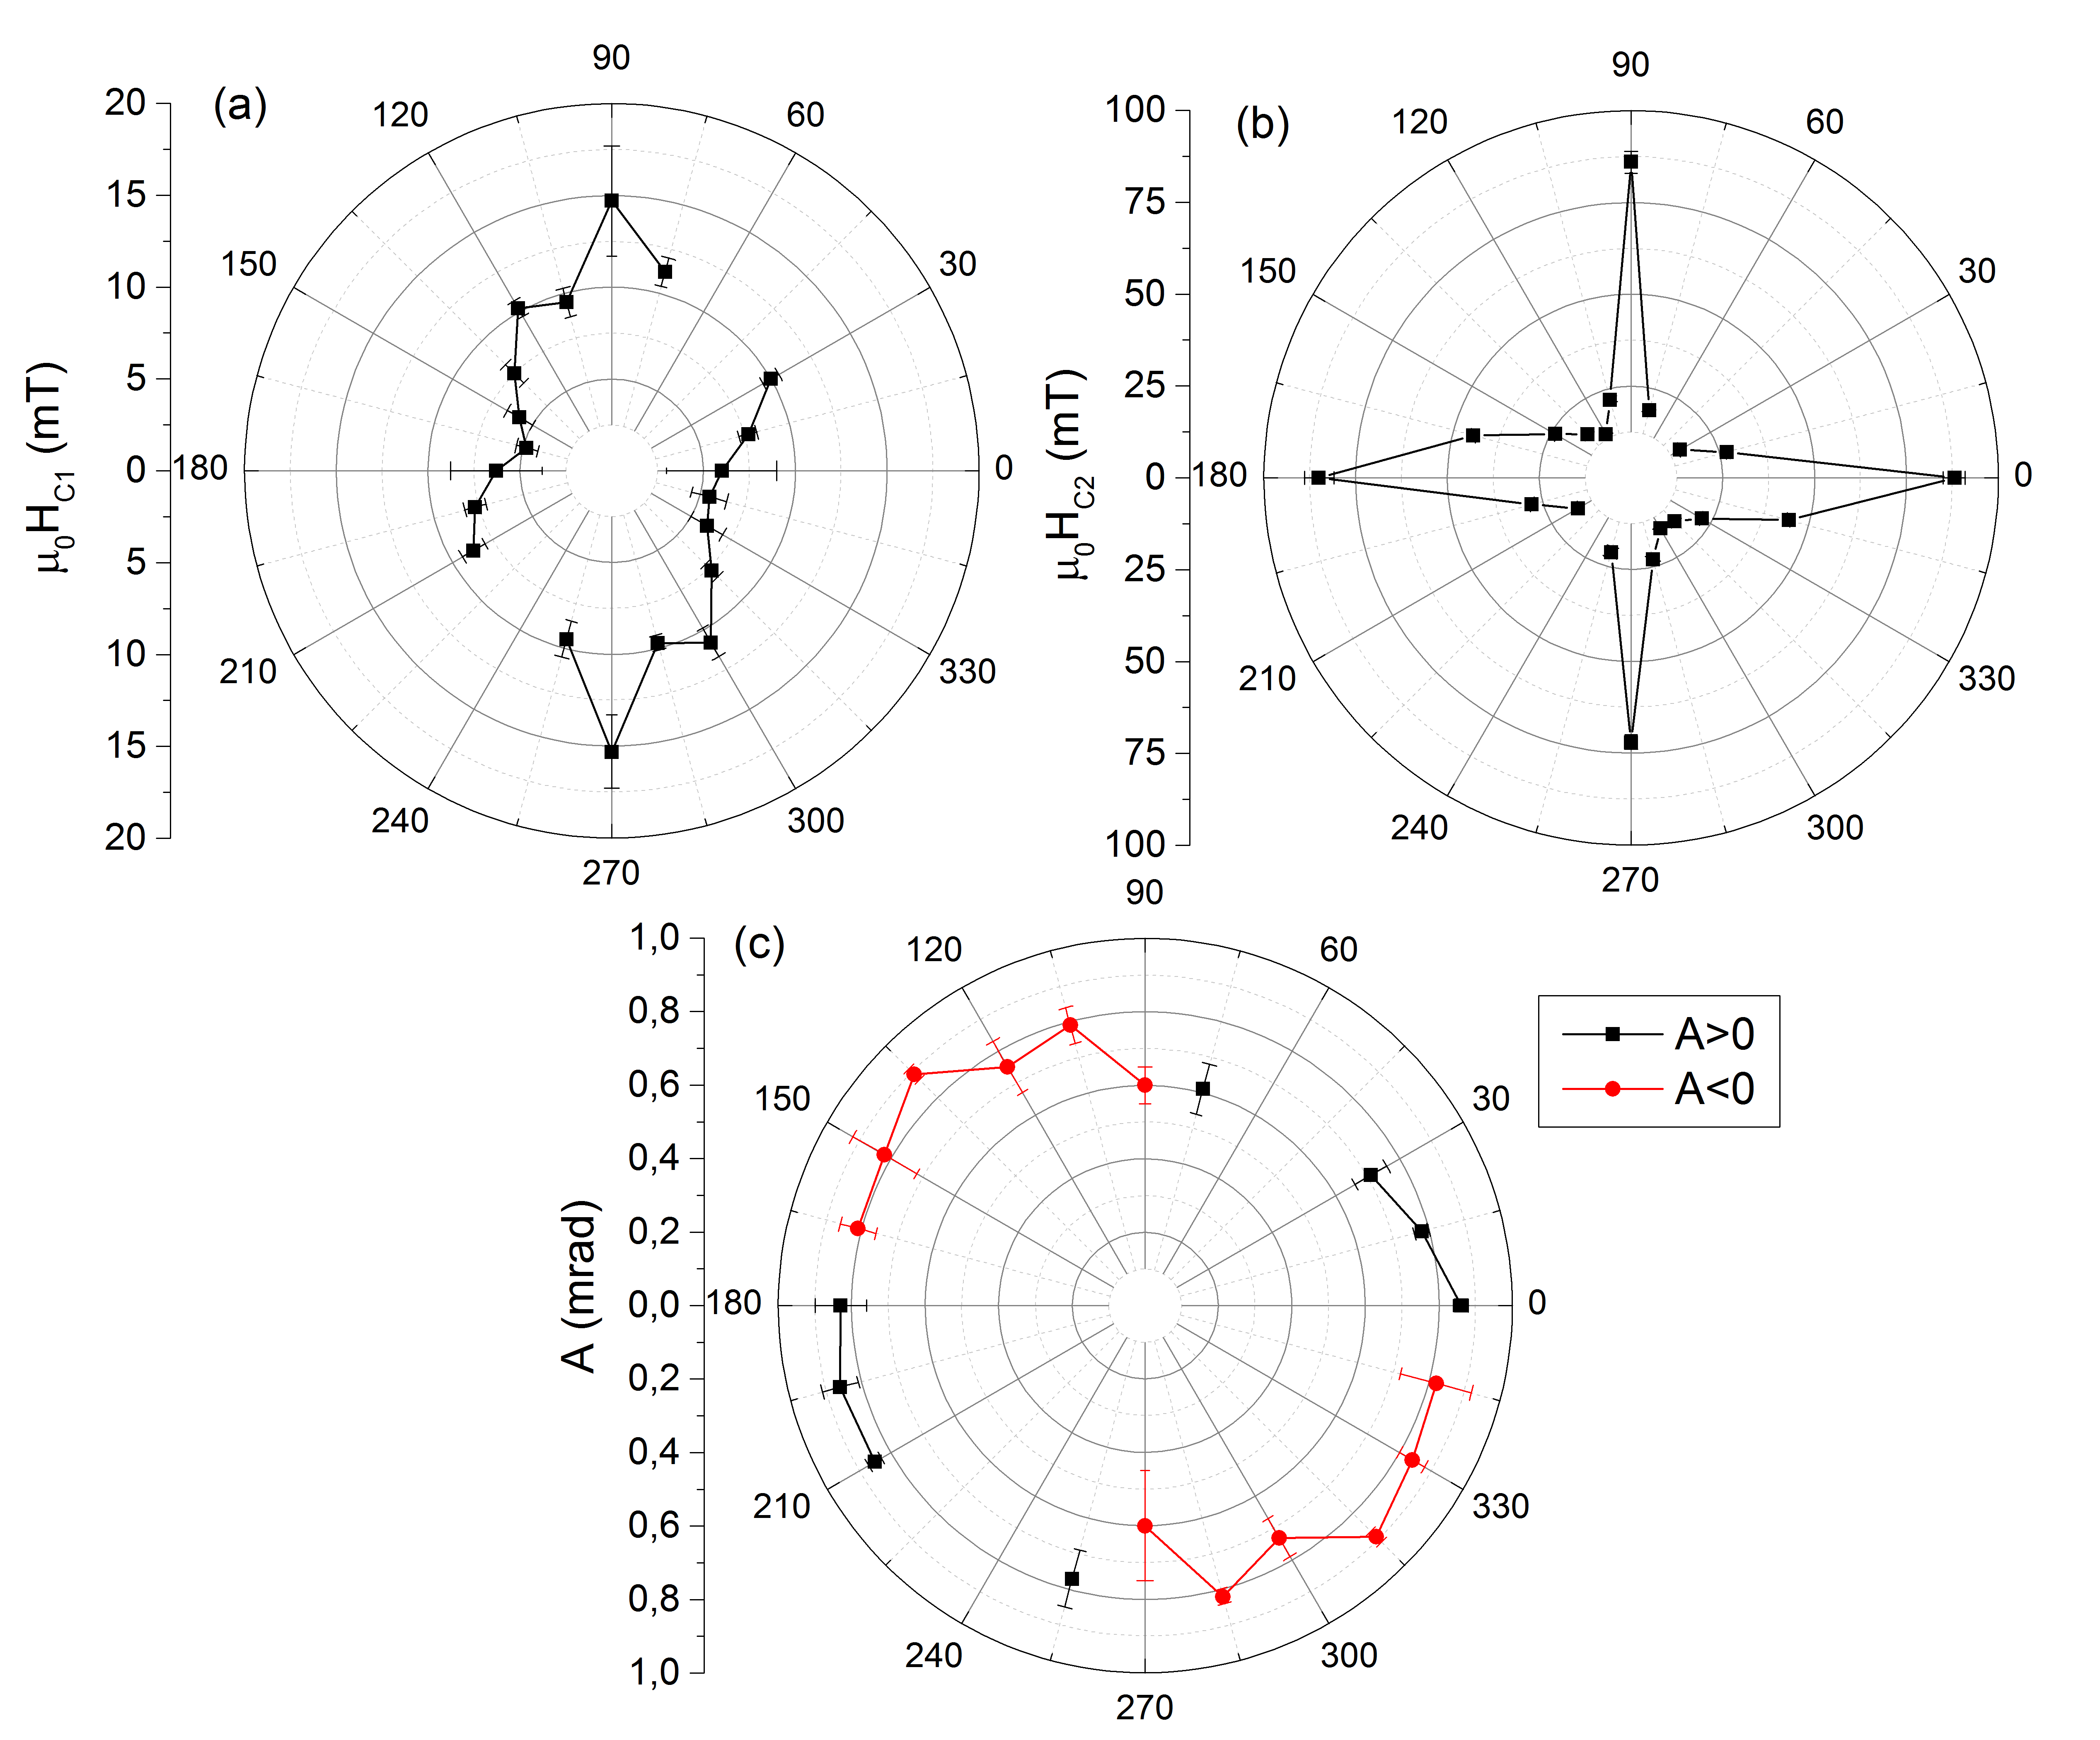
\includegraphics[width=\textwidth]{./png/hystgraf_okolo}}
	\caption{Měření Voigtova jevu v hysterezních smyčkách pro různá $\phH$. (a) Úhlová závislost $\hcj$. (b) Úhlová závislost $\hcd$. (c) Úhlová závislost amplitudy přeskoku $A$. Kladné hodnoty černě, záporné červeně.}\label{kol_okolo}
\end{figure}

Nejzajímavější je graf koercitivních polí $\hcd$, ve kterém jsou jasně patrné významné krystalografické směry [110] a [-110] (porovnejte s \ref{souradna_soustava_vzorek} (b)).



\subsection{Teplotní závislost při vnějším poli ve směru \ang{135}}

Vzorek jsme nejprve zchladili při vypnutém topení ($T=\SI{12(3)}{\kelvin}$). Nastavením teploty na termočlánku jsme vzorek zahřívali s krokem \SI{5}{\kelvin} až do takové teploty, kdy hysterezní smyčky přestaly být patrné. Skutečný rozsah měřených teplot byl 12-\SI{60}{\kelvin}. Intenzita laseru dopadajícího na vzorek byla \SI{2}{\milli\watt}.

Měříme pouze polarizaci $\beta=\ang{0}$, tedy $\gamma-\beta=\ang{90}$.

Teplotní závislost hysterezních smyček je na obr. \ref{kol_vysl_tep_voigt} (a). U hysterezních smyček sledujeme opět veličiny $\hcj$, $\hcd$ a $A$ (viz obr. \ref{kol_vysl_tep_voigt} (b), (c)).


\begin{figure}[htbp]\centering
\qq{	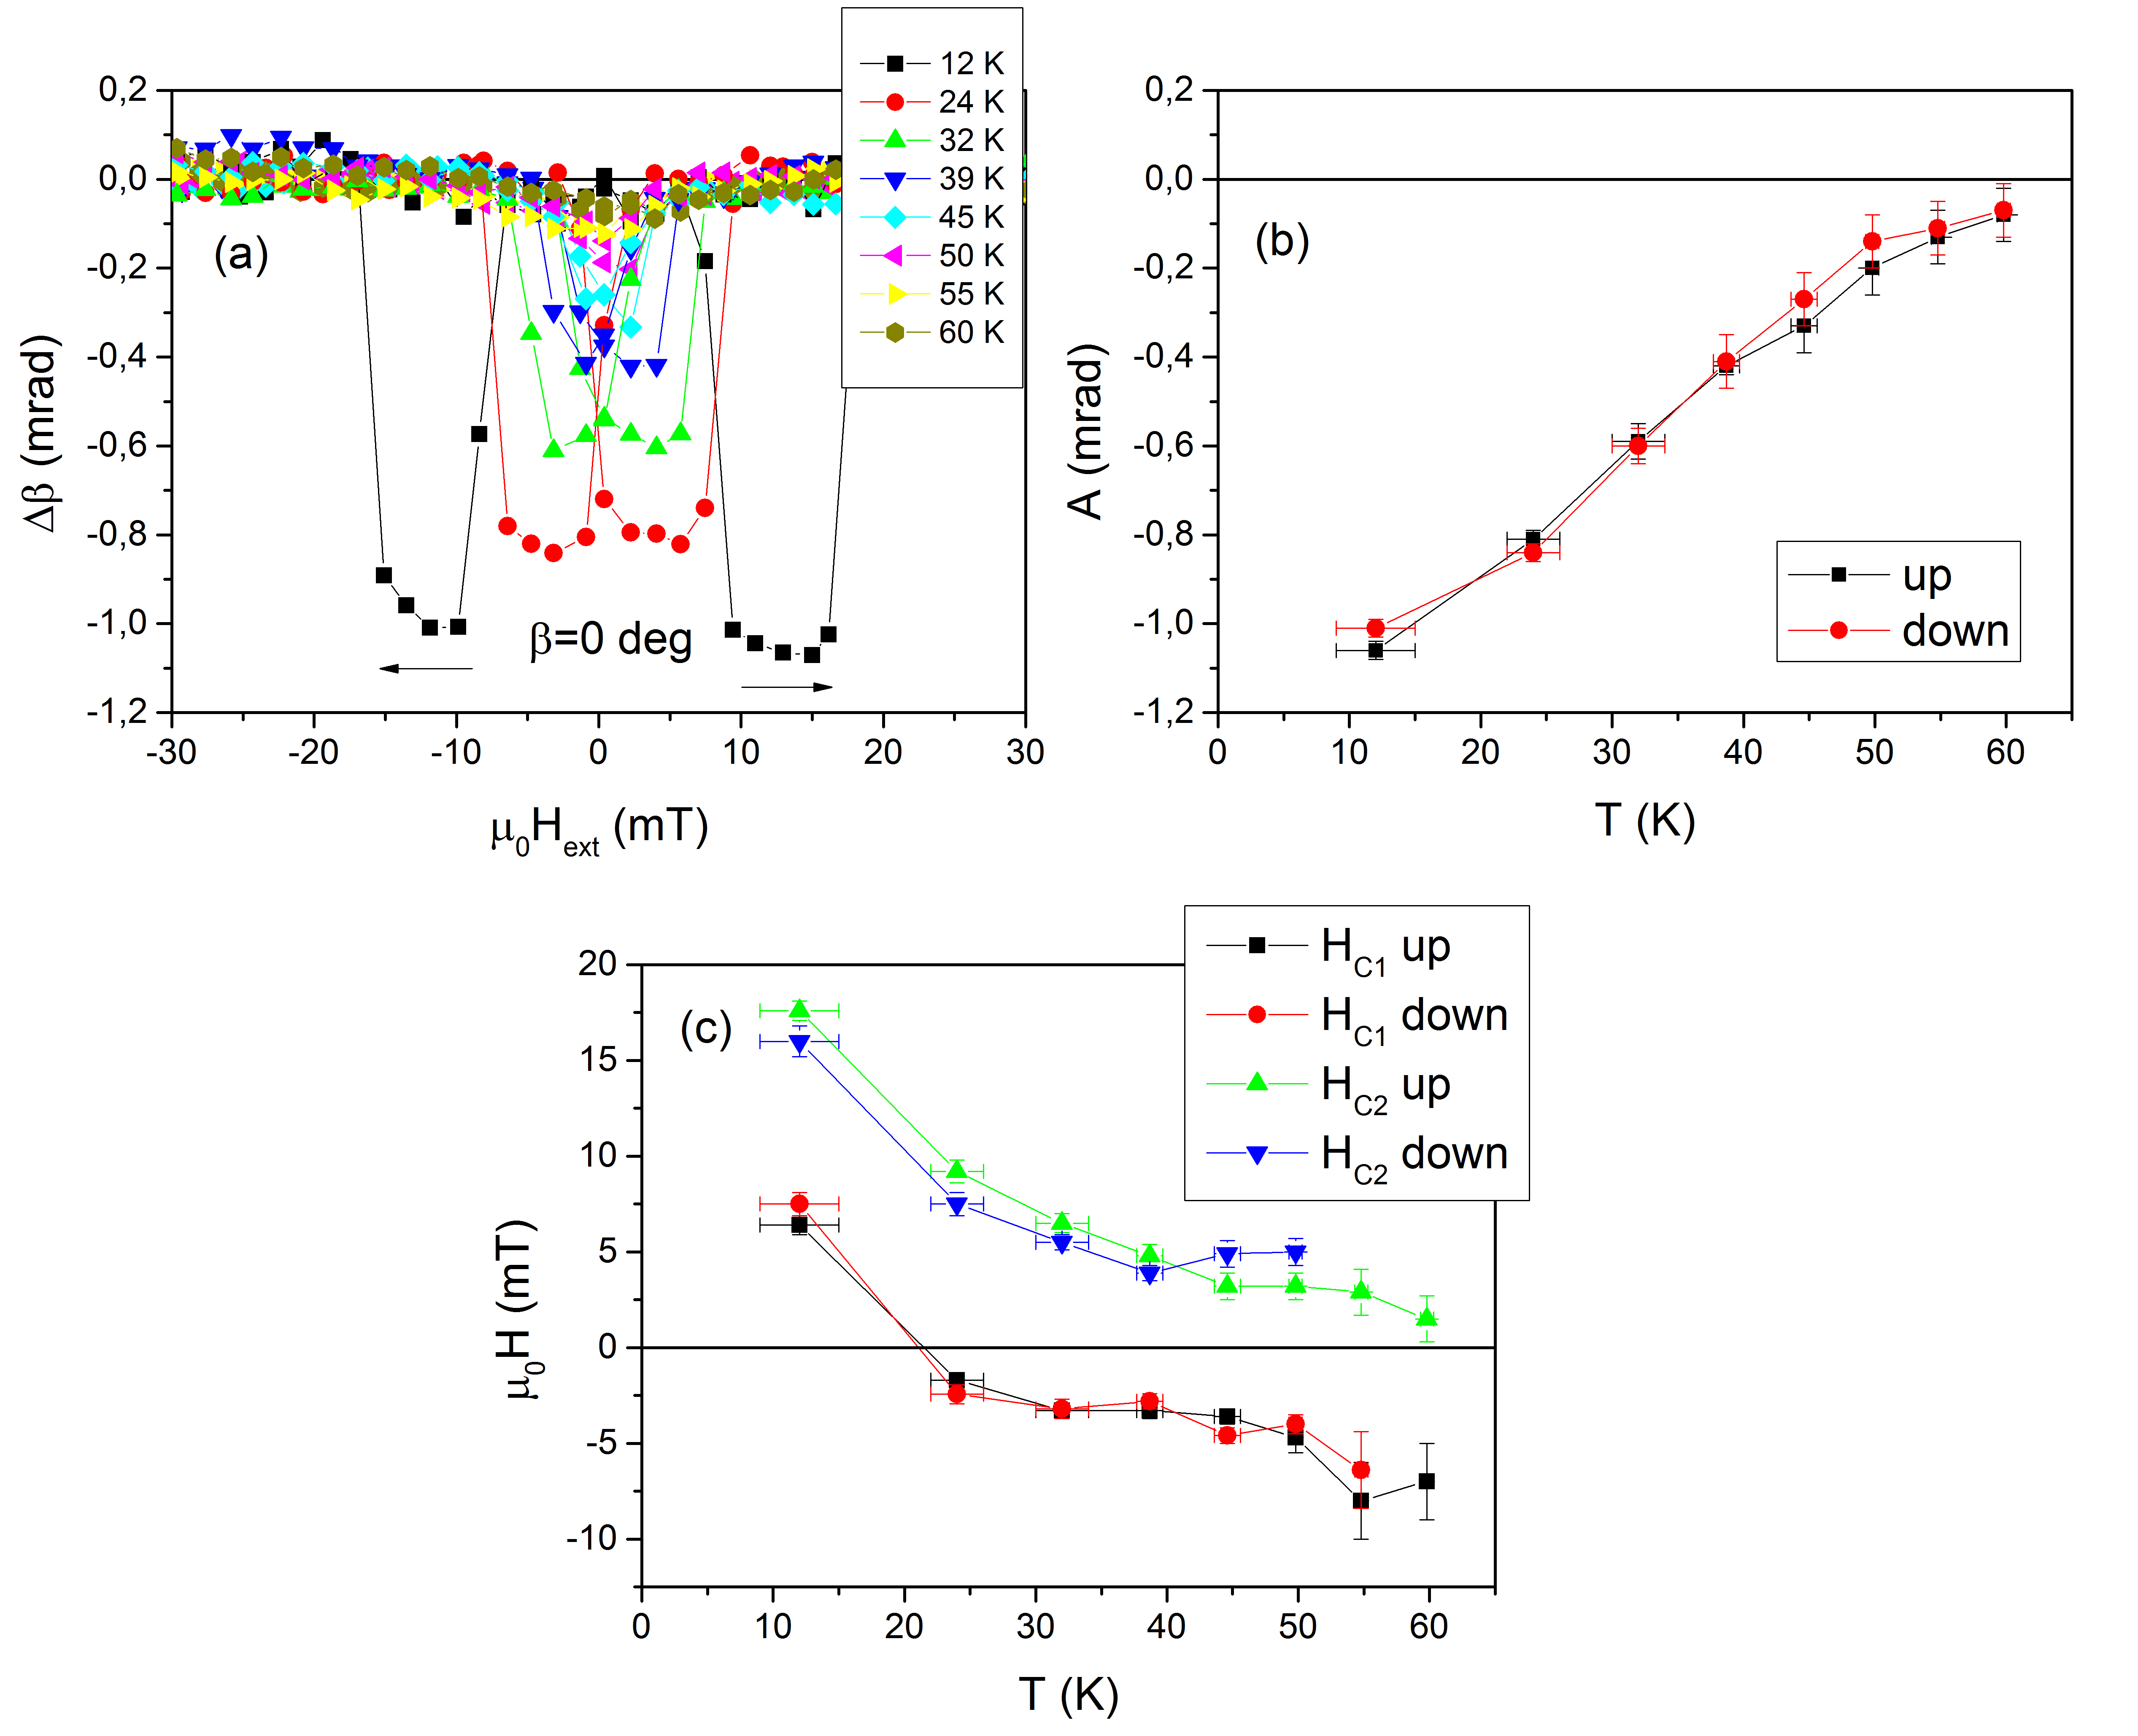
\includegraphics[width=\textwidth]{./png/kolhyst_135tepl}}
	\caption{Měření teplotní závislosti Voigtova jevu v hysterezních smyčkách pro $\phH=\ang{135}$ v kolineární geometrii. (a) Hysterezní smyčky při všech měřených teplotách. (b) Teplotní závislost amplitudy přeskoku $A$. (c) Teplotní závislost koercitivních polí.}\label{kol_vysl_tep_voigt}
\end{figure}
